\section{Sistema Web Django}

El sistema web fue implementado para representar el proceso de un escenario real completo que va desde la inscripción de un alumno a una escuela, la creación de su credencial, hasta su inscripción a un ETS en caso de reprobar alguna asignatura. 

Este sistema no se desplegó en ningun servicio en la nube puesto que para los fines del proyecto no fue necesario. Sin embargo, este sistema se comunica con el servidor Java, el cual contiene todo el backend, del cual hablaremos más adelante.

Este sistema web fue implementado con el framework Django, el cual tradicionalmente se basa en el patrón de arquitectura Modelo-Vista-Plantilla (MTV por sus siglas en inglés). Sin embargo, para este caso en particular, el modelo no se encuentra implementado dentro de Django, ya que, tanto la lógica como la persistencia están completamente administradas por el servidor Java, tal y como se mencionó anteriormente.

Apesar de no seguir fielmente este patrón de arquitectura, en este sistema se adaptó de tal manera en la que la vista (archivos Views) actúa como el controlador, es decir, recibe las peticiones del usuario, consume la API externa y procesa los datos recibidos. Por otro lado, las plantillas (archivos template) generan las páginas HTML que se le mostrarán al usuario, y a su vez, recibe los datos procesados desde la vista.

El tipo de comunicación que se usa en este sistema junto con el servidor Java, es como el de una arquitectura cliente servidor descoplada, en el que el sistema web Django actúa como el cliente, consumiendo servicios por una API REST desarrollada en el servidor mediante peticiones HTTP y con un intercambio de datos en formato JSON.

A continuación, en las figuras \ref{fig:WebForms}, \ref{fig:loginHTML} y \ref{loginView}, se muestran fragmentos del código de cómo está implementado este sistema.

\begin{figure}[H]
	\centering
	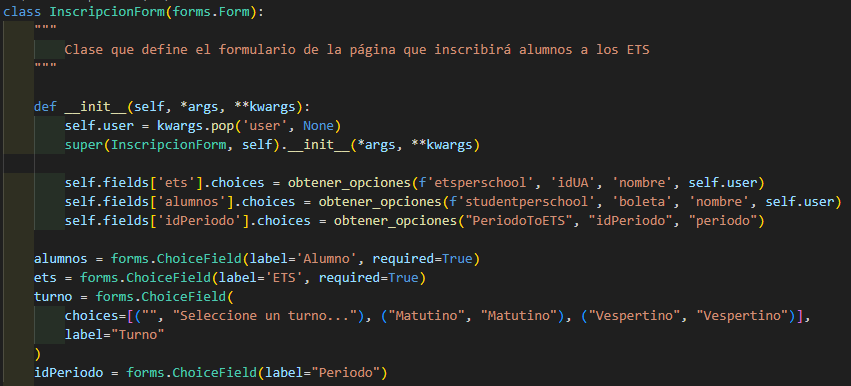
\includegraphics[width=0.7\textwidth]{images/WebForms.png}
	\caption{Definición de campos de formularios.}
	\label{fig:WebForms}
\end{figure}

\begin{figure}[H]
	\centering
	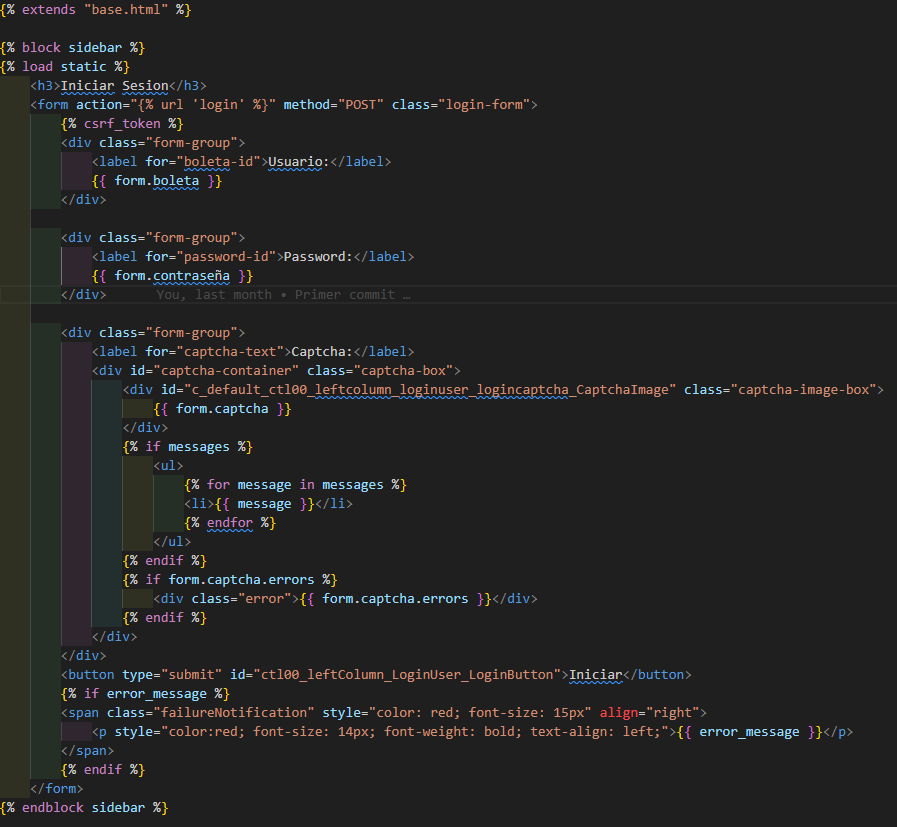
\includegraphics[width=0.7\textwidth]{images/loginHTML.png}
	\caption{Página HTML.}
	\label{fig:loginHTML}
\end{figure}

\begin{figure}[H]
	\centering
	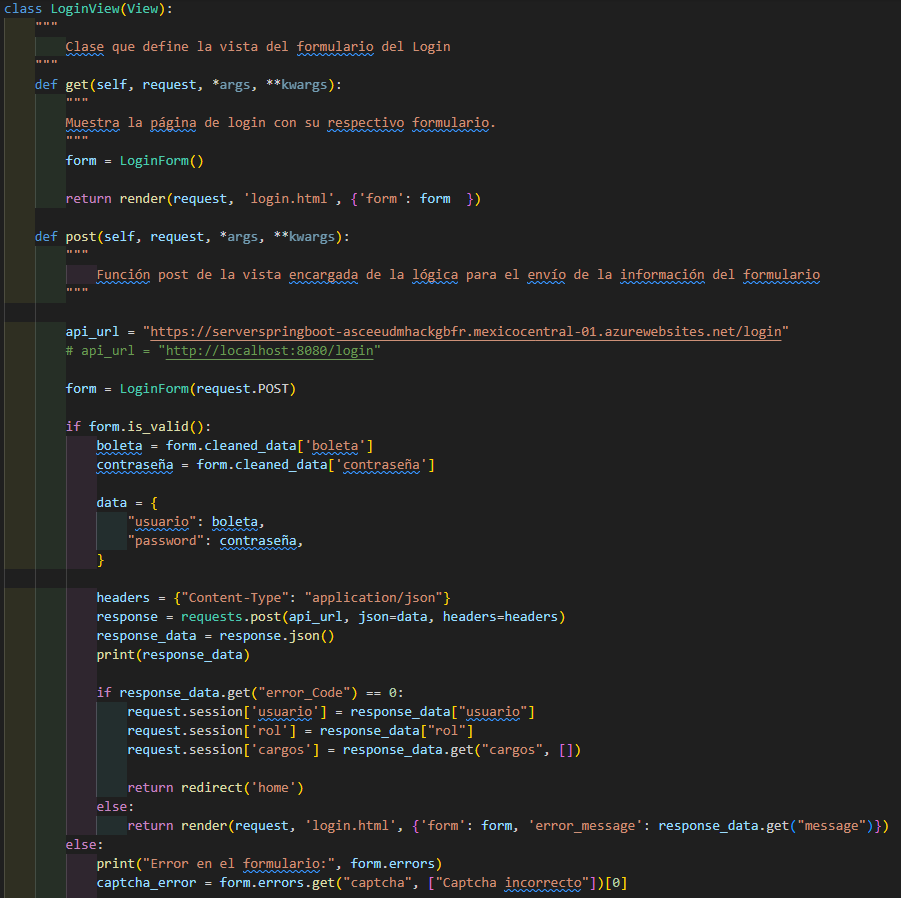
\includegraphics[width=0.7\textwidth]{images/loginView.png}
	\caption{Lógica de interacción con el backend.}
	\label{fig:loginView}
\end{figure}